\chapter{Prime Numbers}\label{chapter:fundamental-theorem-of-arithmetic}

\section{The Fundamental Theorem of Arithmetic}

\begin{definition}
  An integer $a$ is said to be \emph{prime} if it has exactly one positive proper divisor. Any integer $a\neq \pm 1$ that is not prime is said to be a \emph{composite number}.
\end{definition}

The numbers $0$ and $1$ are not prime. To see that $0$ isn't prime, simply note that any positive integer is a proper divisor of $0$. To see that $1$ isn't prime, note that $1$ doesn't have any proper divisors. Indeed, it has exactly one positive divisor, namely $1$ itself, but this divisor isn't proper. We also note that if $a>1$ is prime, then the number $1$ is always a positive proper divisor. Thus we see that $a>1$ is prime if and only if the number $1$ is its unique positive proper divisor.

To see that the number $2$ is prime, note that its positive divisors are a subset of the set $\{1,2\}$ consisting of all the positive integers below $2$. Its proper divisors are therefore a subset of $\{1\}$. The integer $1$ is indeed a positive divisor, so we see that $2$ has exactly one positive proper divisor.

To see that the number $3$ is prime, note that its positive divisors are a subset of the set $\{1,2,3\}$ consisting of all positive integers below $3$. The number $1$ is a proper divisor, the number $2$ doesn't divide $3$, and $3$ itself is a divisor but it isn't proper. Therefore we see that the number $3$ has exactly one positive proper divisor.

The number $4$ isn't prime, because the numbers $1$ and $2$ are two distinct proper divisors of $4$. This process of finding all primes up to a desired bound is formalized in the \emph{sieve of Eratosthenes}, which we will now describe. \cref{figure:sieve-of-eratosthenes} displays the sieve of Eratosthenes up to 1350.

\begin{figure}[!p]
\centering
\resizebox{\textwidth}{!}{%
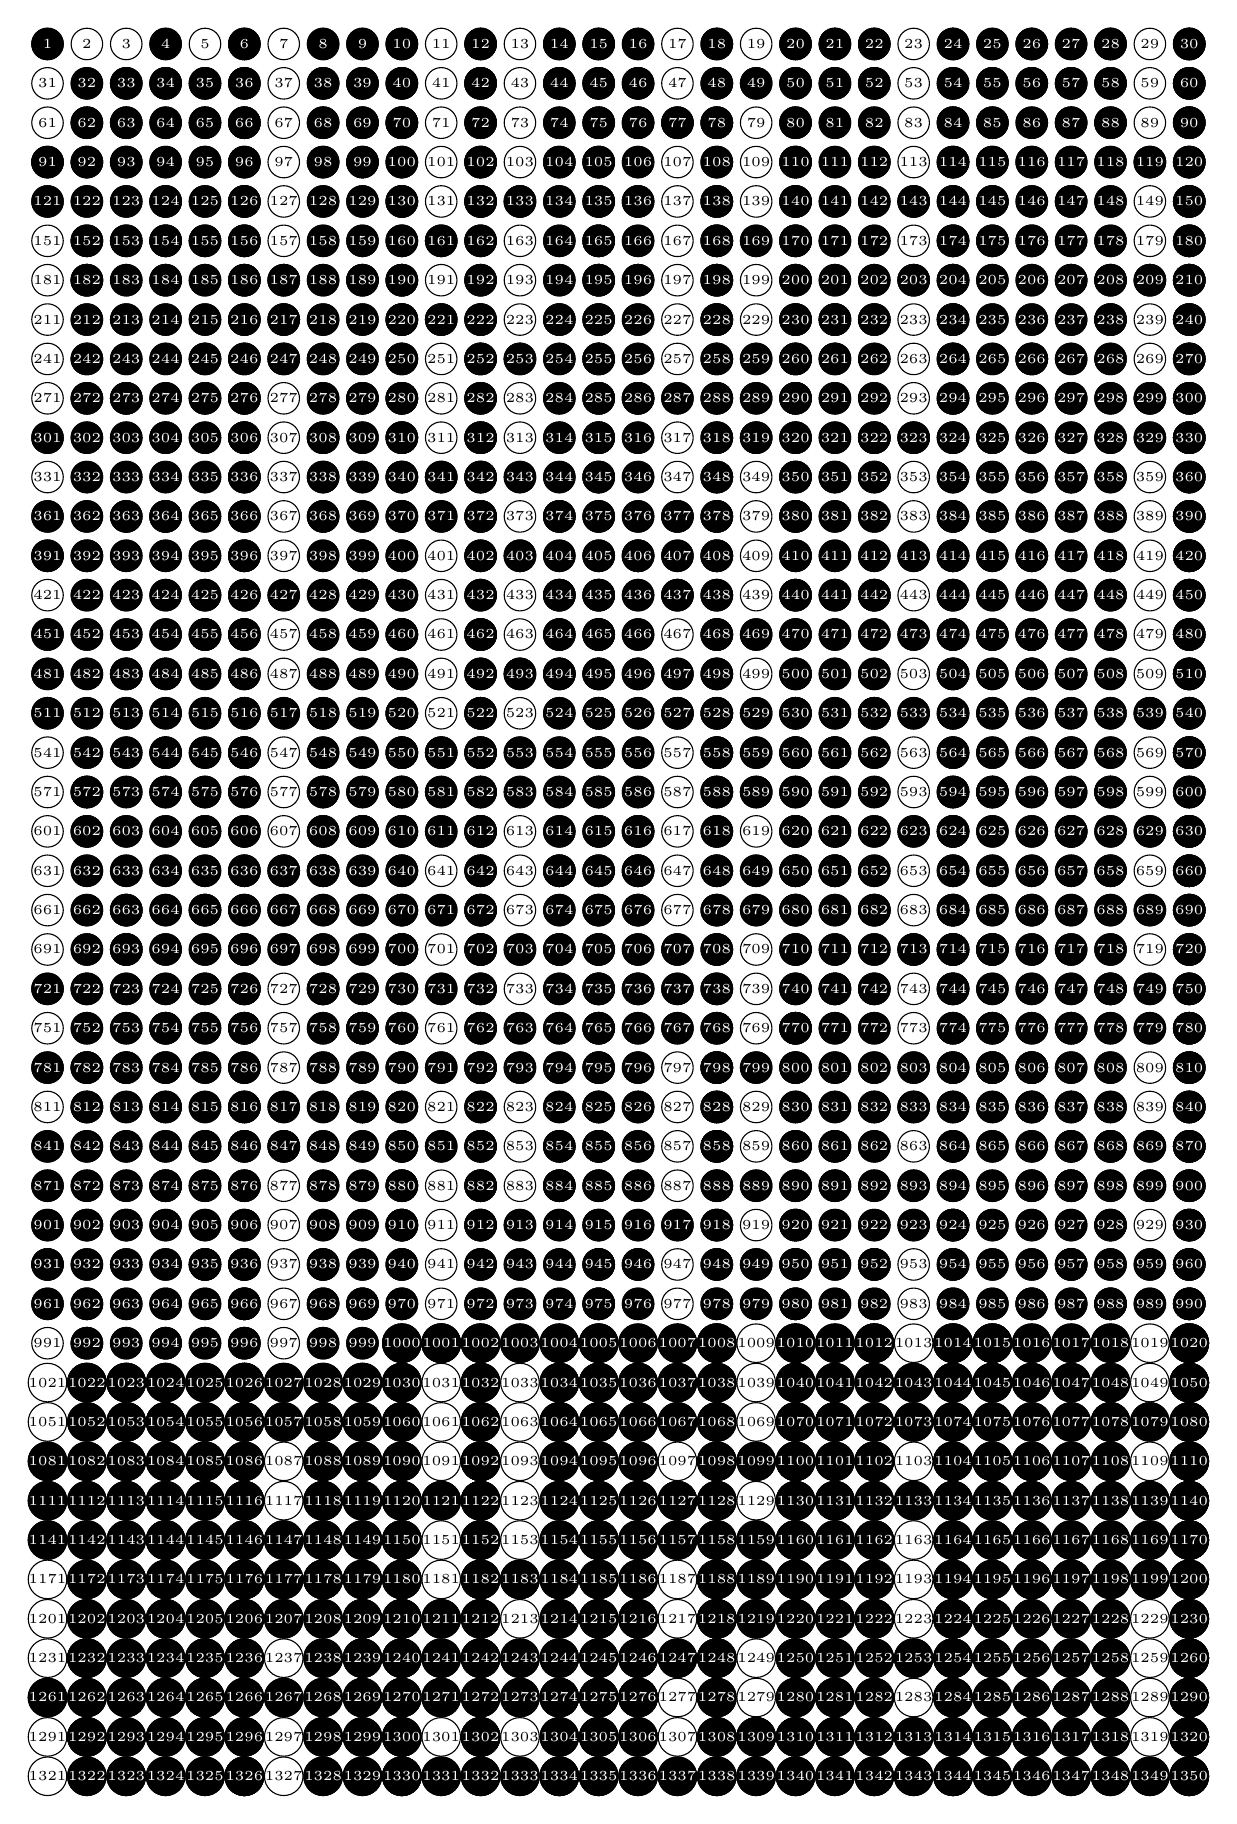
\begin{tikzpicture}[x=0.5cm,y=0.5cm]

  % PARAMETERS
  \def\Cols{30}                       % number of columns
  \def\N{1350}                        % max number
  \pgfmathsetmacro{\Rows}{ceil(\N/\Cols)}  % computed number of rows
  \def\CirDiam{0.4cm}                 % diameter of every circle

  % 1) draw every number in a white circle of fixed size
  \foreach \i in {1,...,\N} {
    \pgfmathtruncatemacro{\c}{mod(\i-1,\Cols)}
    \pgfmathtruncatemacro{\r}{int((\i-1)/\Cols)}
    \node[
      circle,
      draw,
      fill=white,
      minimum size=\CirDiam,
      inner sep=0pt,
      font=\tiny
    ] at (\c+0.5,-\r-0.5) {\i};
  }

  % 2) mark '1' as composite (filled black)
  \node[
    circle,
    draw,
    fill=black,
    text=white,
    minimum size=\CirDiam,
    inner sep=0pt,
    font=\tiny
  ] at (0.5,-0.5) {1};

  % 3) sieve out composites: for each prime ≤ √1350 fill its multiples
  \foreach \p in {2,3,5,7,11,13,17,19,23,29,31} {
    \pgfmathtruncatemacro{\q}{int(1350/\p)}
    \foreach \k in {2,...,\q} {
      \pgfmathtruncatemacro{\m}{\p*\k}
      \ifnum\m>\N
        \breakforeach
      \fi
      \pgfmathtruncatemacro{\cc}{mod(\m-1,\Cols)}
      \pgfmathtruncatemacro{\rr}{int((\m-1)/\Cols)}
      % overwrite with black circle
      \node[
        circle,
        draw,
        fill=black,
        text=white,
        minimum size=\CirDiam,
        inner sep=0pt,
        font=\tiny
      ] at (\cc+0.5,-\rr-0.5) {\m};
    }
  }

\end{tikzpicture}%
}
\caption{\label{figure:sieve-of-eratosthenes}The sieve of Eratosthenes up to 1350: The number 1 and every composite number are marked in black, leaving just the primes in white circles.}
\end{figure}

The sieve of Eratosthenes is an iterative process that generates at stage $n$ a set $P_n$ of numbers known to be prime at stage $n$, and a set $Q_n$ of prime candidates. In other words, the sets $P_n$ form an increasing sequence
\begin{equation*}
  P_0\subseteq P_1\subseteq P_2 \subseteq \cdots
\end{equation*}
of sets of numbers known to be prime, where at each higher stage the set of known primes becomes larger, and the sets $Q_n$ form a decreasing sequence
\begin{equation*}
  Q_0\supseteq Q_1 \supseteq Q_2 \supseteq \cdots
\end{equation*}
of candidates, from which we pick our next prime. We will define the sets $P_n$ and $Q_n$ by a recursive process. Initially, the set $P_0$ is empty and $Q_0=\{n\in\mathbb{N}\mid n\geq 2\}$ is the set of all numbers $\geq 2$. Now we define $P_{n+1}$ to be $P_n\cup \{p(n)\}$, where $p(n):=\min(Q_n)$, and we define
\begin{equation*}
  Q_{n+1}:=Q_n\setminus \{kp(n)\mid k\geq 1\}.
\end{equation*}
In other words, the $n$th prime $p(n)$ is the minimal element of $Q(n)$, and the set $Q_{n+1}$ of candidates is the set $Q_n$ minus all the multiples of $p(n)$. In the first five stages, these sets look as follows:

\begin{center}
  \renewcommand{\arraystretch}{1.2} % Adjust row spacing
  \setlength{\tabcolsep}{10pt}      % Adjust column spacing
  \begin{tabular}{r|l l}
    \textbf{$n$} & \textbf{$P_n$} & \textbf{$Q_n$} \\ \hline
    0 & $\emptyset$ & $\{2,3,4,5,6,7,8,\ldots\}$ \\
    1 & $\{2\}$ & $\{3,5,7,9,11,13,15,\ldots\}$ \\
    2 & $\{2,3\}$ & $\{5,7,11,13,17,19,23,\ldots\}$ \\
    3 & $\{2,3,5\}$ & $\{7,11,13,17,19,23,29,\ldots\}$ \\
    4 & $\{2,3,5,7\}$ & $\{11,13,17,19,23,29,31,\ldots\}$ \\
    5 & $\{2,3,5,7,11\}$ & $\{13,17,19,23,29,31,37,\ldots\}$ \\
  \end{tabular}
\end{center}

Notice that not only the minimal element of $Q_n$ is prime, but every element $q\in Q_n$ such that $q<(\max(P_n))^2$ is prime. This is because if $q<(\max(P_n))^2$ is composite, then its lowest factor must be a prime number $p<\max(P_n)$, i.e., it must be a prime number in $P_n$. However, all the multiples of the primes in $P_n$ have been removed from $Q_n$, so there are no such composite numbers.

We can use this observation to obtain the list of all primes below $100$, at stage $5$ in the sieve of Eratosthenes. The list of primes below $100$ is
\begin{equation*}
2,3,5,7,11,13,17,19,23,29,31,37,41,43,47,53,59,61,67,71,73,79,83,89,97.
\end{equation*}

The sieve of Eratosthenes either terminates, i.e., it reaches a stage for which $Q_n$ is empty, or there are infinitely many primes. We will now show that there are infinitely many primes. In the following lemma we use the concept of \emph{nontrivial divisors}, which are divisors $d$ of a natural number $n$ such that $d\neq 1$. The concept of nontrivial divisors should not be confused with the concept of proper divisors, which are divisors $d$ of a natural number $n$ such that $d\neq n$.

\begin{theorem}
  Any natural number $n>1$ has a least nontrivial divisor, and this divisor is prime.
\end{theorem}

\begin{proof}
  Suppose that $n>1$. Then the set of nontrivial divisors $d\neq 1$ of $n$ contains the number $n$, so it has a least element $p$ by the well-ordering principle of the natural numbers. Then the set of divisors of $p$ itself is the set $\{1,p\}$, because any divisor of $p$ also divides $n$, and $p$ is assumed to be the least nontrivial divisor. This shows that $p$ has exactly one proper divisor, and therefore $p$ is prime.
\end{proof}

The following proposition is due to Euclid, who included it as proposition 30 of book VII of the \emph{Elements}.

\begin{lemma}\label{lemma:cases-prime-divisibility}
  Suppose that $p$ is prime, and that $a$ is an integer. Then either $p\mid a$ or $\gcd(p,a)=1$.
\end{lemma}

\begin{proof}
  The greatest common divisor of $p$ and $a$ is in particular a divisor of $p$, so it is either $1$ or $p$. If $\gcd(p,a)=p$, then we have $p\mid a$.
\end{proof}

\begin{proposition}\label{proposition:euclid-divisibility-primes}
  Consider a positive integer $a$. The following are equivalent:
  \begin{enumerate}
  \item The integer $a$ is prime.
  \item We have $a>1$, and for any two integers $b$ and $c$ such that $a\mid bc$, we have that $a\mid b$ or $a\mid c$.
  \end{enumerate}
\end{proposition}

\begin{proof}
  Suppose first that $a$ is prime. Since $0$ and $1$ aren't prime, it follows that $a>1$. Now consider two integers $b$ and $c$ such that $a\mid bc$. There are two cases to consider: either $a\mid b$, in which case we are done immediately, or $a\nmid b$. In the case where $a\nmid b$, it follows from \cref{lemma:cases-prime-divisibility} that $a$ and $b$ are relatively prime. This allows us to apply \cref{proposition:coprime-divides-product}, by which we conclude that $a\mid c$.

  For the converse, suppose that for any two integers $b$ and $c$ such that $a\mid bc$, we have $a\mid b$ or $a\mid c$, and let $d$ be a proper divisor of $a$. Now consider any positive proper divisor $d$ of $a$, and write $a=dk$. Then it follows in particular that $a \mid dk$, so by assumption we have either $a\mid d$ or $a\mid k$. The first condition can be ruled out, because $d$ is assumed to be a proper divisor and therefore $a \nmid d$. Thus we find ourselves in the second case, where $a\mid k$ and $k\mid a$. The integer $k$ is also positive, since $a$ and $d$ are positive, so it follows that $a=k$. This implies that $d=1$, and hence we conclude that $a$ is prime.
\end{proof}

\begin{theorem}\label{theorem:fundamental-theorem-of-arithmetic}
  For any natural number $n>0$, there is a unique list $\ell=(p_0,\ldots,p_{l-1})$ of length $l$, consisting of primes $p_0\leq p_1\leq \cdots \leq p_{l-1}$ such that
  \begin{equation*}
    n=\prod_{i=0}^{l-1}p_i.
  \end{equation*}
  This unique list of primes is called the \emph{prime decomposition of $n$}.
\end{theorem}

\begin{proof}
  We apply strong induction on $n$, with base case $1$. In the base case, we let $\ell$ be the empty list. The empty list satisfies the increasing primes condition vacuously, and empty products are $1$ by definition, so the empty list is indeed a prime decomposition of $1$.

  For the inductive step, recall that any natural number $n+1>1$ has a least prime divisor. If $p$ is the least prime divisor of $n+1$, then it follows that $(n+1)/p\leq n$. By the strong induction hypothesis we have a unique prime decomposition $(q_0,\ldots,q_{l-1})$ of $(n+1)/p$. Now define the list $\ell:=(p_0,p_1,\ldots,p_l)$ by $p_0:=p$ and $p_{i+1}:=q_i$. Then each $p_i$ is a prime divisor of $n+1$, and since $p_0$ is the least prime divisor of $n+1$ we have the inequalities
  \begin{equation*}
    p_0\leq p_1 \leq \cdots \leq p_l.
  \end{equation*}
  Furthermore, we have
  \begin{equation*}
    n+1 = p\cdot ((n+1)/p) = p_0 \cdot \prod_{i=1}^l p_i = \prod_{i=0}^l p_i.
  \end{equation*}
  This proves that the prime decomposition of $n+1$ exists.

  To show that the prime decomposition of $n+1$ is unique, let $(r_0,\cdots,r_k)$ be a prime decomposition of $n+1$. The smallest prime divisor $p$ of $n+1$ then divides the product
  \begin{equation*}
    p \mid \prod_{i=0}^k r_i.
  \end{equation*}
  This implies that $p\mid r_i$ for some $0\leq i \leq k$, i.e., that $p=r_i$. However, $p$ is assumed to be the smallest prime factor of $n+1$, so it follows that $p=r_0$. Now it follows that $(r_1,\ldots,r_k)$ is a prime decomposition of $(n+1)/p$, which is unique, and therefore we conclude that $n+1$ has a unique prime factorization.
\end{proof}

\section{The Infinitude of Primes}

The theorem asserting the infinitude of primes asserts that no finite set of primes is the set of all primes. Many proofs of the infinitude of primes require the following lemma:

\begin{lemma}
  If $a$ and $b$ are relatively prime integers, then any prime divisors of $a$ are distinct from any prime divisors of $b$.
\end{lemma}

\begin{proof}
  Suppose that $a$ and $b$ are relatively prime, and that $p$ and $q$ are prime divisors of $a$ and $b$, respectively. By the assumption that $a$ and $b$ are relatively prime, it follows that $p\nmid b$ and that $q\nmid a$. Therefore it follows that $p$ and $q$ cannot be the same.
\end{proof}

\begin{theorem}\label{theorem:infinitude-of-primes}
  There are infinitely many prime numbers.
\end{theorem}

\begin{proof}[Euclid's proof of \cref{theorem:infinitude-of-primes}]
  We will prove that there are infinitely many prime numbers by showing that for any finite set of prime numbers, there is a prime number not belonging to the finite set.
  
  Consider a finite set $\{p_0,\ldots,p_k\}$ of primes, and define
  \begin{equation*}
    n:= 1+\prod_{i=0}^k p_i
  \end{equation*}
  Then there exists, for each $0\leq i\leq k$, a natural number $q_i$ such that $n=q_ip_i+1$. Indeed, we can simply define
  \begin{equation*}
    q_i := \prod_{j=0,j\neq i}^k p_j.
  \end{equation*}
  Since $n$ can be written in this way, it follows that $n$ is relatively prime to each $p_i$. Consequently, the least prime divisor of $n$ is relatively prime to each $p_i$. In other words, the least prime divisor of $n$ is not in the set of primes $\{p_0,\ldots,p_k\}$.
\end{proof}

\subsection{Saidak's Proof}

There are many proofs of the infinitude of primes. The following is due to Filip Saidak \cite{Saidak2006}, who published his proof in 2006, based on the idea that if $n=ab$ is the product of two numbers that are relatively prime and both at least $2$, then $n$ must have two prime factors.

\begin{proof}[Saidak's proof of \cref{theorem:infinitude-of-primes}]
  Let $N_0:= 1$, and define
  \begin{equation*}
    N_{n+1} := N_n(N_n + 1).
  \end{equation*}
  We claim that $N_n$ has at least $n$ prime factors. In the base case, we note that it is indeed true that $1$ has at least zero prime factors. For the inductive step, suppose that $N_n$ has at least $n$ prime factors. The number $N_n+1$ is relatively prime to $N_n$, so its prime factors are all distinct from the prime factors of $N_n$. Furthermore, we have $1<N_n+1$, so $N_n+1$ indeed has at least one prime factor. Thus it follows that $N_{n+1}$ has at least $n+1$ prime factors, and therefore there must be infinitely many primes.
\end{proof}

\subsection{Goldbach's Proof}

Our next proof of the infinitude of primes is due to Goldbach, from 1730. In the 18th century, it was customary among mathematicians to share their findings private correspondences. In July of 1730, Goldbach wrote a letter to Euler, in which he established that all distinct Fermat numbers are relatively prime, and that hence there must be infinitely many primes.

Recall that the Fermat numbers $\Phi_n$ are defined by
\begin{equation*}
  \Phi_n := 2^{2^n}+1.
\end{equation*}

\begin{theorem}[Goldbach's Theorem]\label{theorem:goldbachs-theorem}
  Any two distinct Fermat numbers are relatively prime.
\end{theorem}

\begin{proof}
  Consider two distinct natural numbers $m$ and $n$, and assume that $m<n$. Recall from \cref{exercise:product-formula-fermat-numbers} that
  \begin{equation*}
    \Phi_n-2 = \prod_{k<n}\Phi_k.
  \end{equation*}
  Thus we see that $\Phi_m \mid \Phi_n - 2$. It follows that any common divisor $d$ of $\Phi_m$ and $\Phi_n$ is also a divisor of $2$, i.e., $d=1$ or $d=2$. However, all Fermat numbers are clearly odd, and this implies that any common divisor of $\Phi_m$ and $\Phi_n$ is $1$. In other words, $\Phi_m$ and $\Phi_n$ are relatively prime.
\end{proof}

\begin{proof}[Goldbach's proof of \cref{theorem:infinitude-of-primes}]
  Since any two distinct Fermat numbers are relatively prime, and since any number $n>1$ has a prime divisor, it follows that if we pick a prime divisor of each Fermat number $\Phi_n$, then we picked infinitely many distinct prime numbers.
\end{proof}

\subsection{Furstenberg's Proof, Following Cass--Wildenberg}

The following proof of the infinitude of primes is, in its essence, due to Hillel Furstenberg \cite{furstenberg1955}. In its original formulation, this proof makes clever use of a topology on $\mathbb{Z}$. Although topologies are not hard to define, motivating them is beyond the scope of this course. We will therefore present a revised version of Furstenberg's proof, following Daniel Cass and Gerald Wildenberg \cite{cass2003}.

The Cass--Wildenberg approach to prove the infinitude of primes makes use of the concept of a periodic subset of $\mathbb{Z}$. A subset $A\subseteq\mathbb{Z}$ is said to be \emph{periodic with period $n$}, or simply \emph{periodic} if we merely assume such a natural number $n$ to exist, if we have
\begin{equation*}
  x\in A\qquad\Leftrightarrow\qquad x+n\in\mathbb{Z}.
\end{equation*}
Thus, if $A$ is a periodic subset of $\mathbb{Z}$ with period $n$, and $x\in A$, then
\begin{equation*}
  x+kn\in A
\end{equation*}
for all $k\in\mathbb{Z}$. In particular, all inhabited periodic subsets of $\mathbb{Z}$ are infinite. We note two basic facts about periodic subsets of $\mathbb{Z}$, which we leave to the reader to verify:
\begin{enumerate}
\item If $A_1,\ldots,A_m$ is a finite family of periodic subsets of $\mathbb{Z}$, each with their own periods, then the union
  \begin{equation*}
    A_1\cup\cdots\cup A_m
  \end{equation*}
  is again a periodic subset of $k$. The period of the union is the least common multiple of the periods of the subsets $A_i$.
\item If $A$ is a periodic subset of $\mathbb{Z}$, then its complement $\complementsubset{A} :=\{x\in\mathbb{Z}\mid x\notin A\}$ is periodic with the same period.
\end{enumerate}

\begin{proof}[The Furstenberg proof of \cref{theorem:infinitude-of-primes}, following Cass--Wildenberg]
  Consider the subsets
  \begin{equation*}
    S_p:=\{kp\mid k\in\mathbb{Z}\},
  \end{equation*}
  where $p$ is a prime number, and define
  \begin{equation*}
    S:=\bigcup_{p\,\mathrm{prime}}S_p.
  \end{equation*}
  Since every integer besides $\pm 1$ is divisible by a prime, it follows that $S$ consists of all the integers besides $\pm 1$. The complement of $S$ is therefore the set $\{-1,1\}$. Note that the subset $\{-1,1\}$ of $\mathbb{Z}$ cannot be periodic, since is inhabited and finite. This allows us to conclude that the subset $S$ of $\mathbb{Z}$ is not periodic. However, if there were only finitely many primes, then $S$ would be periodic because it would be a finite union of periodic subsets of $\mathbb{Z}$. Thus we conclude that there must be infinitely many primes.
\end{proof}

\subsection{Erd\H{o}s's Proof}

\begin{definition}
  A natural number $n$ is said to be \emph{square-free} if the only square dividing $n$ is $1$. In other words, $n$ is square-free if
  \begin{equation*}
    k^2\mid n\qquad\Rightarrow\qquad k=1
  \end{equation*}
  for every natural number $k$.
\end{definition}

By the \crefnamed{theorem:fundamental-theorem-of-arithmetic}{Fundamental Theorem of Arithmetic} it follows that square-free numbers are those numbers of which the prime decomposition
\begin{equation*}
  n=p_1\cdots p_n
\end{equation*}
is a product of distinct primes. In particular, if $n$ is square free then the exponents in the prime factorization of $n$ do not exceed $1$. For instance, the numbers $3\cdot 5\cdot 17$ and $2\cdot 11\cdot 37$ are square-free, while the numbers $3^3\cdot 5\cdot 31$ and $2^5\cdot 5^{11}\cdot 61$ aren't.

\begin{theorem}\label{theorem:square-free-decomposition}
  Every natural number $n$ can be written uniquely in the form
  \begin{equation*}
    n=k^2m
  \end{equation*}
  where $m$ is a square-free number. This is called the \emph{square-free decomposition} of $n$, and the number $m$ is called the \emph{square-free part} of $n$.
\end{theorem}

\begin{proof}
  Consider the set of natural numbers
  \begin{equation*}
    S := \{d\in\mathbb{N}\mid\text{There exists a $k\in\mathbb{N}$ such that $k^2d=n$}\}.
  \end{equation*}
  Clearly, this set contains the element $n$ itself, since $n/n=1$ is a perfect square. By the \crefnamed{theorem:well-ordering-natural-numbers}{Well-Ordering Principle}, it follows that $S$ has a least element, which we call $m$. By definition, $n/m$ is a perfect square, so there is a natural number $k$ such that
  \begin{equation*}
    n=k^2m.
  \end{equation*}
  Next, we need to show that $m$ is square-free. Suppose $d^2\mid m$ is a positive divisor of $m$. Then the quotient $q=m/d^2$ is a divisor of $n$ such that $n/q$ is the perfect square $(kd)^2$. Since $q\leq m$ it follows by minimality that $q=m$ and hence that $d^2=1$. This implies that $d=1$.

  To finish the proof, we need to show that the square-free decomposition of $n$ is unique. To this end, suppose that $n=l^2d$, where $d$ is square-free. We claim that any prime divisor of $k$ is a prime divisor of $l$ and conversely that any prime divisor of $l$ is a prime divisor of $k$. To see this, note that for any prime $p\mid k$ we have $p^2\mid k^2$ and consequently $p^2\mid l^2d$. Since $d$ is square-free, this implies that $p\mid l^2$ and hence that $p\mid l$. The same argument applies the other way around, so it follows that $k=l$ and consequently $m=d$.
\end{proof}

Now that we have established that every natural number has a unique square-free decomposition, we are able to give Erd\H{o}s's proof of the infinitude of primes. This proof was originally published in \cite{erdos1938}.

\begin{proof}[Erd\H{o}s's proof of \cref{theorem:infinitude-of-primes}]
  Consider a finite list of primes $p_1,\ldots,p_n$. We claim that for any $x$, there are at most
  \begin{equation*}
    \sqrt{x}2^n
  \end{equation*}
  numbers below $x$ with all prime factors from the list $p_1,\ldots,p_n$. To see this, recall from \cref{theorem:square-free-decomposition} that any number can be written in the form $k^2m$ where $m$ is square free. Then we have $k\leq\sqrt{x}$, leaving at most $\sqrt{x}$ choices for the number $k$. Furthermore, there are only $2^n$ square-free numbers $m$ whose prime factors are from the list $p_1,\ldots,p_n$, leaving at most $2^n$ choices for the value of $m$.
  
  If all the numbers below $x$ are products of powers of primes from the list $p_1,\ldots,p_n$, we find that $x\leq\sqrt{x}2^n$, or equivalently that
  \begin{equation*}
    \sqrt{x}\leq 2^n
  \end{equation*}
  However, this inequality clearly fails when $x$ exceeds $2^{2n}$, so there must be primes other than $p_1,\ldots,p_n$.
\end{proof}

\section{Legendre's Formula and Kummer's Theorem}

In some cases we can give precise expressions of the prime factorization of a number. We will describe here two such cases: The prime factorization of the factorial $n!$, which is due to Adrien-Marie Legendre, and the prime factorization of the binomial coefficients $\binom{n}{m}$, which is due to Ernst Kummer. These explicit formulas will be useful in the study of the distribution of the primes.

\begin{definition}
  The \emph{$p$-adic valuation} of a positive integer $n$ is the largest exponent $m$ such that $p^m\mid n$. That is, it is the unique natural number $m$ such that
  \begin{equation*}
    p^k\mid n\qquad\Leftrightarrow\qquad k\leq m
  \end{equation*}
  for every natural number $k$. We will write $\nu_p(n)$ for the $p$-adic valuation of $n$.
\end{definition}

For example, the $2$-adic valuation of $24$ is $\nu_2(24)=3$ because the exponent of $2$ in $24=2^3\cdot 3$ is $3$, and its $3$-adic valuation is $\nu_3(24)=1$ because the exponent of $3$ in $2^3\cdot 3$ is $1$. Another useful fact is that the $p$-adic valuation of the greatest common divisor of two numbers is the minimum of their respective $p$-adic valuations. More generally, if the greatest common divisor is taken of multiple natural numbers we obtain
\begin{equation*}
  \nu_p(\gcd(n_1,\ldots,n_k))=\min(\nu_p(n_1),\ldots,\nu_p(n_k)).
\end{equation*}
Likewise, the $p$-adic valuation of the least common multiple of $n_1,\ldots,n_k$ is
\begin{equation*}
  \nu_p(\lcm(n_1,\ldots,n_k))=\max(\nu_p(n_1),\ldots,\nu_p(n_k)).
\end{equation*}
For example the greatest common divisor and the least common multiple of $60=2^2\cdot 3\cdot 5$ and $525=3\cdot 5^2\cdot 7$ are
\begin{equation*}
  \gcd(60,525)=3\cdot 5=15\qquad\text{and}\qquad\lcm(60,525)=2^2\cdot 3\cdot 5^2\cdot 7=2100.
\end{equation*}

\begin{theorem}[Legendre's formula]\label{theorem:legendres-formula}
  For any natural number $n$, we have
  \begin{equation*}
    n!=\prod_{p\leq n}p^{\left\lfloor\frac{n}{p}\right\rfloor + \left\lfloor\frac{n}{p^2}\right\rfloor + \cdots}.
  \end{equation*}
\end{theorem}

\begin{proof}
  Another way of stating Legendre's formula for $n!$ is that the $p$-adic valuation of $n!$ is given by
  \begin{equation*}
    \nu_p(n!) = \sum_{k=1}^\infty\left\lfloor\frac{n}{p^k}\right\rfloor.
  \end{equation*}
  To see this, note that each integer $1\leq x \leq n$ divisible by $p$ contributes a factor $p$ to $n!$. Each integer $1\leq x\leq n$ divisible by $p^2$ contributes a second factor of $p$ to $n!$, and more generally, each integer $1\leq x \leq n$ divisible by $p^k$ contributes a $k$th factor of $p$.

  Since there are $\bigl\lfloor\frac{n}{p^k}\bigr\rfloor$ integers from $1$ to $n$ divisible by $p^k$, it follows that the number of factors of $p$ in $n!$ is
  \begin{equation*}
    \sum_{k=1}^\infty\left\lfloor\frac{n}{p^k}\right\rfloor.\qedhere
  \end{equation*}
\end{proof}

Incidentally, Legendre's formula can be used to give yet another proof of the infinitude of primes, due to Junho Peter Whang \cite{whang2010}.

\begin{proof}[Whang's proof of \cref{theorem:infinitude-of-primes}]
  The $p$-adic valuation of $n!$ is bounded from above by
  \begin{equation*}
    \nu_p(n!)= \sum_{k=1}^{\infty}\left\lfloor\frac{n}{p^k}\right\rfloor \leq \sum_{k=1}^{\infty}\frac{n}{p^k}=\frac{n}{p-1}.
  \end{equation*}
  Now suppose that $n$ is a natural number so that all the primes below $n$ are from the list $p_1,\ldots,p_m$, and define
  \begin{equation*}
    M := \prod_{i=1}^mp_i^{\frac{1}{p_i-1}}.
  \end{equation*}
  Then it follows from Legendre's formula that
  \begin{equation*}
    n!\leq M^n.
  \end{equation*}
  To give a quick lower bound for $n!$, note that for $1\leq k\leq n$ we have $n\leq k(n+1-k)$. This gives the inequalities
  \begin{equation*}
    n^{\frac{n}{2}}\leq n! \leq M^n.
  \end{equation*}
  However, this inequality fails when $n$ exceeds $M^2$, so it follows that for $n>M^2$ there must be a prime not in the list $p_1,\ldots,p_m$.
\end{proof}

In the following theorem we give a useful alternative expression for the $p$-adic valuation of $n!$.

\begin{theorem}[de Polignac's formula]\label{theorem:de-polignacs-formula}
  Consider a natural number $n\geq 1$ written in its base $p$ representation
  \begin{equation*}
    \sum_{i=0}^{l} a_ip^i,
  \end{equation*}
  where we have $0\leq a_i<p$ for each $i$. Then $p$-adic valuation of $n!$ is
  \begin{equation*}
    \nu_p(n!) = \frac{n-\sum_{i=0}^{l} a_i}{p-1}.
  \end{equation*}
\end{theorem}

\begin{proof}
  Given the base-$p$ representation of $n$, the base-$p$ representation of $\lfloor\frac{n}{p^k}\rfloor$ is given by dropping the digits first $k$ digits in the base-$p$ representation of $n$:
  \begin{equation*}
    \left\lfloor\frac{n}{p^k}\right\rfloor = a_k + a_{k+1}p +\cdots + a_lp^{l-k}.
  \end{equation*}
  Using this observation, we obtain:
  \begin{equation*}
    \sum_{k=1}^{l}\left\lfloor\frac{n}{p^k}\right\rfloor
    = \sum_{k=1}^{l}\sum_{j=k}^{l}a_jp^{j-k}
    = \sum_{j=1}^la_j\sum_{k=1}^{j}p^{j-k}
    = \sum_{j=1}^la_j\frac{p^j-1}{p-1}.
  \end{equation*}
  On the other hand, we have
  \begin{equation*}
    n-\sum_{j=0}^l a_j = \sum_{j=0}^l a_jp^j-a_j = \sum_{j=0}^l a_j(p^j-1).
  \end{equation*}
  This gives
  \begin{equation*}
    \frac{n-\sum_{j=0}^l a_j}{p-1} = \sum_{j=0}^l a_j\frac{p^j-1}{p-1}=
    \sum_{k=1}^{l}\left\lfloor\frac{n}{p^k}\right\rfloor.\qedhere
  \end{equation*}
\end{proof}

\begin{example}
  We can use Legendre's formula and de Polignac's formula to compute the prime factorizations of binomial coefficients. For example, it follows immediately from Legendre's formula that all the prime factors of the central binomial coefficient
  \begin{equation*}
    \binom{64}{32}
  \end{equation*}
  are bounded from above by $64$. Moreover, every prime $32<p\leq 64$ occurs with $p$-adic valuation $1$. Furthermore, the central binomial coefficient $\binom{64}{32}$ is not divisible by any prime $\frac{2}{3}32<p\leq 32$, showing that the $23$-, $29$-, and $31$-adic valuations of $\binom{64}{32}$ are $0$. To compute the $p$-adic valuations for the lower primes, we use de Polignac's formula, for which it is necessary to write $32$ and $64$ in base $p$. Using letters $A$, $B$, $C$, and so forth for digits representing values of $10$ and higher, we gather all the calculations for de Polignac's formula in the following table:
  \begin{center}
    \begin{tabular}{c|ccc}
      $p$ & $32$ base $p$ & $64$ base $p$ & $\frac{2s_p(32)-s_p(64)}{p-1}$ \\ \midrule
      $2$ & $(100000)_2$ & $(1000000)_2$ & $1$ \\
      $3$ & $(1012)_3$ & $(2101)_3$ & $2$ \\
      $5$ & $(112)_5$ & $(224)_5$ & $0$ \\
      $7$ & $(44)_7$ & $(121)_7$ & $2$ \\
      $11$ & $(2A)_{11}$ & $(59)_{11}$ & $1$ \\
      $13$ & $(26)_{13}$ & $(4C)_{13}$ & $0$ \\
      $17$ & $(1F)_{17}$ & $(3D)_{17}$ & $1$ \\
      $19$ & $(1D)_{19}$ & $(37)_{19}$ & $1$ \\
    \end{tabular}
  \end{center}
  Thus, we see that
  \begin{equation*}
    \binom{64}{32}=2\cdot 3^2\cdot 7^2\cdot 11\cdot 17\cdot 19\cdot 37\cdot 41\cdot 43\cdot 47\cdot 53\cdot 59\cdot 61.
  \end{equation*}
  Even though the binomial coefficient $\binom{64}{32}$ is a fairly large number with $19$ decimal digits, we didn't need to evaluate it in order to obtain its prime factorization. In fact, without fully evaluating it, we can now determine the last decimal digit of $\binom{64}{32}$ by the following procedure: Start with $d_0:=1$ and let $d_{i+1}$ be the remainder of the product $d_ip_i^{m_i}$ after division by $10$, where $p_i^{m_i}$ is the $i$th prime power in the prime factorization of $\binom{64}{32}$. This gives:
  \begin{equation*}
    d_1 = 2,~d_2=8,~d_3=2,~d_4=2,~\ldots,~d_{13}=4.
  \end{equation*}
  The last decimal digit of $\binom{64}{32}$ is therefore a $4$.
\end{example}

In the following theorem, which is due to Ernst Kummer \cite{kummer1852}, we will compute the $p$-adic valuation of the binomial coefficients in full generality. Before we do this, we need to recall addition of two natural numbers written in base $p$. Suppose that
\begin{equation*}
  m=\sum_{i=0}^{l_m}a_ip^i\qquad\text{and}\qquad n=\sum_{i=0}^{l_{n}}b_ip^i.
\end{equation*}
Then their sum $m+n$ has base-$p$ representation
\begin{equation*}
  m+n=\sum_{i=0}^{l_n}c_ip^i,
\end{equation*}
where $c_i$ is obtained by the following recursive procedure, simultaneously with a number $u(m,n)_i\in\{0,1\}$ recording whether a $1$ needs to be carried over to the next digit: Set $u(m,n)_0=0$ and define
\begin{equation*}
  (c_i,u(m,n)_{i+1}) :=
  \begin{cases}
    (a_i+b_i+u(m,n)_i,0) & \text{if }a_i+b_i+u(m,n)_i< p \\
    (a_i+b_i+u(m,n)_i-p,1) & \text{if }a_i+b_i+u(m,n)_i\geq p.
  \end{cases}
\end{equation*}

\begin{theorem}[Kummer's Theorem]\label{theorem:kummers-theorem}
  Consider two natural numbers $m$ and $n$. The $p$-adic valuation of the binomial coefficient $\binom{m+n}{m}$ is the number of carries in the addition of $m$ and $n$ in base $p$: If $m$ and $n$ have base $p$-representations
  \begin{equation*}
    m = \sum_{i=0}^{l_m}a_ip^i\qquad\text{and}\qquad n = \sum_{i=0}^{l_n}b_ip^i,
  \end{equation*}
  then
  \begin{equation*}
    \nu_p\binom{m+n}{m} = \#\{0\leq i \leq l_n \mid u(m,n)_i=1\}.
  \end{equation*}
\end{theorem}

\begin{proof}
  Write $s_p(x)$ for the sum of the digits of the $p$-adic representation of natural number $x$. By de Polignac's formula for the $p$-adic valuation of $(m+n)!$ we find that
  \begin{equation*}
    \nu_p\binom{m+n}{m} = \nu_p((m+n)!)-\nu_p(m!)-\nu_p(n!) =
    \frac{s_p(m)+s_p(n)-s_p(m+n)}{p-1}.
  \end{equation*}
  The $p$-adic representation of $m+n$ is given by
  \begin{equation*}
    m+n = \sum_{i=0}^{l_{m+n}}c_ip^i,
  \end{equation*}
  where
  \begin{equation*}
    c_i =
    \begin{cases}
      a_i+b_i + u(m,n)_i & \text{if } a_i+b_i+u(m,n)_i<p \\
      a_i+b_i + u(m,n)_i - p & \text{otherwise}.
    \end{cases}
  \end{equation*}
  We therefore find that the numerator in de Polignac's expression for $\nu_p\binom{m+n}{m}$ contains a term $p-u(m,n)_{i+1}$ for every time $u(m,n)_{i+1}=1$. That is, the numerator is of the form $C(p-1)$ where $C$ is the number of carries. This proves the theorem.
\end{proof}

Kummer's theorem can be used to show that the binomial coefficient $\binom{n}{k}$ always divides the least common multiple of $1,2,\ldots,n$. In order to prove this result, note that the largest exponent $m$ such that $p^m\leq n$ is the number
\begin{equation*}
  m=\lfloor \log_p(n)\rfloor.
\end{equation*}
In other words, if $m$ is the largest integer not exceeding $\log_p(n)$, then the leading digit in the base-$p$ representation of $n$ belongs to $p^m$. 

\begin{corollary}\label{corollary:kummers-theorem}
  For any $0\leq k\leq n$ we have
  \begin{equation*}
    \binom{n}{k}\,\,\Big|\,\,\lcm(1,\ldots,n).
  \end{equation*}
\end{corollary}

\begin{proof}
  Suppose that the base-$p$ representation of $n$ is
  \begin{equation*}
    n=\sum_{i=0}^{l}a_ip^i.
  \end{equation*}
  Then there are clearly at most $l$ carries when we add $k$ to $n-k$. Since $p^l\leq n$, it follows that
  \begin{equation*}
    p^{\nu_p\binom{n}{k}}\mid\lcm(1,\ldots,n).
  \end{equation*}
  Since this is true for every prime $p\leq n$, and $\binom{n}{k}$ contains only prime divisors up to $n$, the claim follows.
\end{proof}

\section{Bertrand's Postulate}

In 1845, Joseph Bertrand observed that for any $1\leq n \leq 3,000,000$ there is always a prime between $n$ and $2n$, and conjectured that this must be true for all $n$ \cite{bertrand1845}. Nowadays on a computer, it is really easy to generate lists of primes $p_i$ so that the prime $p_{i+1}$ is strictly below $2p_i$ for each $i$. Taking each time the largest possible prime satisfying this requirement, we obtain the list
\begin{align*}
  &2,\ 3,\ 5,\ 7,\ 13,\ 23,\ 43,\ 83,\ 163,\ 317,\ 631,\ 1259,\\
  &2503,\ 5003,\ 9973,\ 19937,\ 39869,\ 79699,\ 159389,\\
  &318751,\ 637499,\ 1274989,\ 2549951,\ 5099893,\ \ldots.
\end{align*}

The primes in this list are sometimes called the \emph{Bertrand primes}, and they are listed as A006992 in the On-Line Encyclopedia of Integer Sequences \cite{oeis:A006992}. Bertrand's conjecture was proven five years later by Pafnuty Chebyshev, who contributed many more results about the distribution of the primes using analytical methods \cite{chebyshev1850}. We will give a proof by Paul Erd\H{o}s \cite{erdos1932}, which can be obtained through the methods of the previous section.

\begin{lemma}\label{lemma:upper-bound-product-of-primes}
  For any positive integer $n$, we have
  \begin{equation*}
    \prod_{p\leq n}p< 4^n.
  \end{equation*}
\end{lemma}

\begin{proof}
  The proof is by induction on $n$. For $n=1$, there are no primes $p\leq 1$, so the product over all the primes $p\leq 1$ is just $1$, which is indeed strictly below $4$. Likewise, the theorem holds for $n=2$, because $2<4^2$.

  For the inductive step, assume that $\prod_{p\leq n}p<4^n$. In order to show that
  \begin{equation*}
    \prod_{p\leq n+1}p < 4^{n+1},
  \end{equation*}
  there are two cases to consider: Either $n+1$ is even or $n+1$ is odd. The even case is immediate: We have
  \begin{equation*}
    \prod_{p\leq n+1}p = \prod_{p\leq n}p < 4^n < 4^{n+1}.
  \end{equation*}
  In the odd case, there is an $m$ such that $2m+1=n+1$. Since every prime $m+2\leq p \leq 2m+1$ divides the binomial coefficient $\binom{2m+1}{m}$, it follows that
  \begin{equation*}
    \prod_{p\leq 2m+1}p\leq \binom{2m+1}{m}\cdot \prod_{p\leq m+1}p < \binom{2m + 1}{m} 4^{m+1}.
  \end{equation*}
  To finish the proof, it suffices to show that $\binom{2m+1}{m}\leq 4^m$. This follows, since the binomial coefficients $\binom{2m+1}{m}$ and $\binom{2m+1}{m+1}$ occur separately in the expansion of $(1+1)^{2m+1}$. However, they are equal, so neither of them can exceed $\frac{1}{2} 2^{2m+1}=4^m$, which proves the lemma.
\end{proof}

\begin{theorem}
  For any positive integer $n$, there is a prime $n<p\leq 2n$.
\end{theorem}

\begin{proof}
  Consider an integer $n\geq 2$ for which there is no prime $n<p<2n$, and let $p$ be a prime divisor of the central binomial coefficient $\binom{2n}{n}$. Such a prime divisor must then be less than or equal to $\frac{2}{3}n$, since $q^3\nmid (2n)!$ for any prime $\frac{2}{3}n<q\leq n$, while $q^2\mid (n!)^2$.

  Now, if $m$ is the largest exponent such that $p^m\mid \binom{2n}{n}$, then it follows from \cref{corollary:kummers-theorem} that
  \begin{equation*}
    p^m\leq 2n.
  \end{equation*}
  This allows us to estimate the number of primes for which $p^2\mid \binom{2n}{n}$. Indeed, if $m\geq 2$, then it follows that
  \begin{equation*}
    p \leq \sqrt[\raisebox{0.3ex}{${\scriptscriptstyle m}$}]{2n}\leq \sqrt{2n}.
  \end{equation*}
  This shows that there are at most $\sqrt{2n}$ primes in the prime factorization of $\binom{2n}{n}$, of which the exponent is larger than $1$. It follows that
  \begin{equation*}
    \frac{4^n}{2n+1}<\binom{2n}{n}\leq (2n)^{\sqrt{2n}}\prod_{p\leq 2n/3}p< (2n)^{\sqrt{2n}} 4^{\frac{2n}{3}},
  \end{equation*}
  where the first inequality was established in \cref{exercise:estimates-central-binomial-coefficients}, and the last inequality follows from \cref{lemma:upper-bound-product-of-primes}. Rearranging this strict inequality, we obtain
  \begin{equation*}
    4^{\frac{n}{3}}<(2n+1)(2n)^{\sqrt{2n}}<(2n)^{\sqrt{2n}+1}.
  \end{equation*}
  Taking logarithms base $2$ on both sides, we find that
  \begin{equation*}
    \frac{n}{2}<\frac{2n}{3} < (\sqrt{2n}+1)\log_2(2n)
  \end{equation*}
  We see that this strict inequality fails for $n\geq 2^9=512$, since
  \begin{equation*}
    2^8 = 512 \nless 330 = (2^5+1)\cdot 10.
  \end{equation*}
  We conclude that Bertrand's postulate must be true for all $n\geq 512$. Using the sieve of Eratosthenes up to 1350, as displayed in \cref{figure:sieve-of-eratosthenes}, we see that the Bertrand primes are indeed primes up to $631$, which is sufficient and thus the theorem is proven.
\end{proof}

\begin{exercises}
  \exercise \label{exercise:shading} In the number grid provided at the end of the introduction, shade the numbered cells in two colors:
  \begin{enumerate}
  \item Leave all the prime numbers unshaded.
  \item Shade the number $1$ and all square-free composite numbers in one color.
  \item Shade all non-square-free numbers in the other color.
  \end{enumerate}
  Explain your method.
  \exercise Compute the square-free decompositions of $72$, $200$, $315$, $462$, and $2205$.
  \exercise Show that there are no primes $p$ such that $p+8$ and $p+22$ are also prime.
  \exercise Show that
  \begin{equation*}
    p\,\,\Big|\,\, \binom{p}{k}
  \end{equation*}
  for any $0<k<p$, and any prime number $p$.
  \exercise Show that
  \begin{equation*}
    4^{\frac{p-1}{2}}\equiv 1\pmod{p}
  \end{equation*}
  for any odd prime number $p$.
  \exercise Define the $n$th \emph{Mersenne number} $M_n$ to be
  \begin{equation*}
    M_n:=2^n-1.
  \end{equation*}
  Show that if $n$ is composite, then so is $M_n$. Conclude that if $M_n$ is prime, then so is $n$. Prime numbers of the form $M_p$ for some prime number $p$ are called \emph{Mersenne primes}.
  \exercise A natural number $n$ is said to be \emph{perfect} if it is the sum of its proper divisors. Show that an even number is perfect if and only if it is of the form $2^{p-1}M_p$, where $M_p$ is a Mersenne prime.
  \exercise Consider a fixed set $\{p_1,\ldots,p_n\}$ of $n$ distinct primes. Given a natural number $k$, how many numbers can be written as a product
  \begin{equation*}
    p_1^{m_1}\cdots p_n^{m_n}
  \end{equation*}
  such that $m_1+\cdots +m_n=k$?
  \exercise Suppose that $n\geq 3$ and $p$ is a prime such that $\frac{2}{3}n<p\leq n$. Prove that
  \begin{equation*}
    p\nmid \binom{2n}{n}.
  \end{equation*}
  \exercise Prove the following identity due to Bakir Farhi \cite{farhi2009}:
  \begin{equation*}
    \lcm\left(\binom{n}{0},\binom{n}{1},\ldots,\binom{n}{n}\right)=
    \frac{\lcm(1,\ldots,n+1)}{n+1}.
  \end{equation*}
  \exercise Determine the number of trailing zeros in the decimal representations of $100!$ and $2^{10}!$.
  \exercise
  \begin{subexenum}
  \item Show that $\binom{n}{m}$ is odd if and only if there are no carries occur when adding $m$ and $n-m$ in their binary representations.
  \item Show that $\binom{n}{m}$ is odd for every $0\leq m\leq n$ if and only if $n$ is of the form $2^k-1$.
  \end{subexenum}
  
\end{exercises}

%%% Local Variables:
%%% mode: latex
%%% TeX-master: "elementary-number-theory"
%%% End:
